
\section{Analysing Predictions: {\normalfont\normalsize Find two interesting audio files that have not been used for training and qualitatively evaluate your classifier’s predictions.}}
\label{sec:Analysing Predictions}

For this task, we use the predictions from our best performing classifier, namely the Logistic Regression model with 'C=0.1, penalty=l2, solver=lbfgs'.\\
We analyze predictions for the two files: 584022.wav, where the model does a good job and 74790.wav, where the struggles with its classifications. \\
For the calculation of prediction quality metrics we skipped class-labels which are not present in the file. Otherwise, some of the misclassifications would actually boost the final Balanced Accuracy.


\subsection{Use the spectrogram and the sequence of predictions to visualize the classifier output. }
\label{sec:Analysing Predictions:a}
We get simply get the model outputs for frames of a single file together with the corresponding 'melspectrogram' feature. We then only plot labels which have been predicted to be present somewhere within the file, see \hyperref[fig:6_plots]{Figure~\ref*{fig:6_plots}}.

\begin{figure}[htbp]
  \centering
  \begin{subfigure}[b]{0.49\textwidth}
    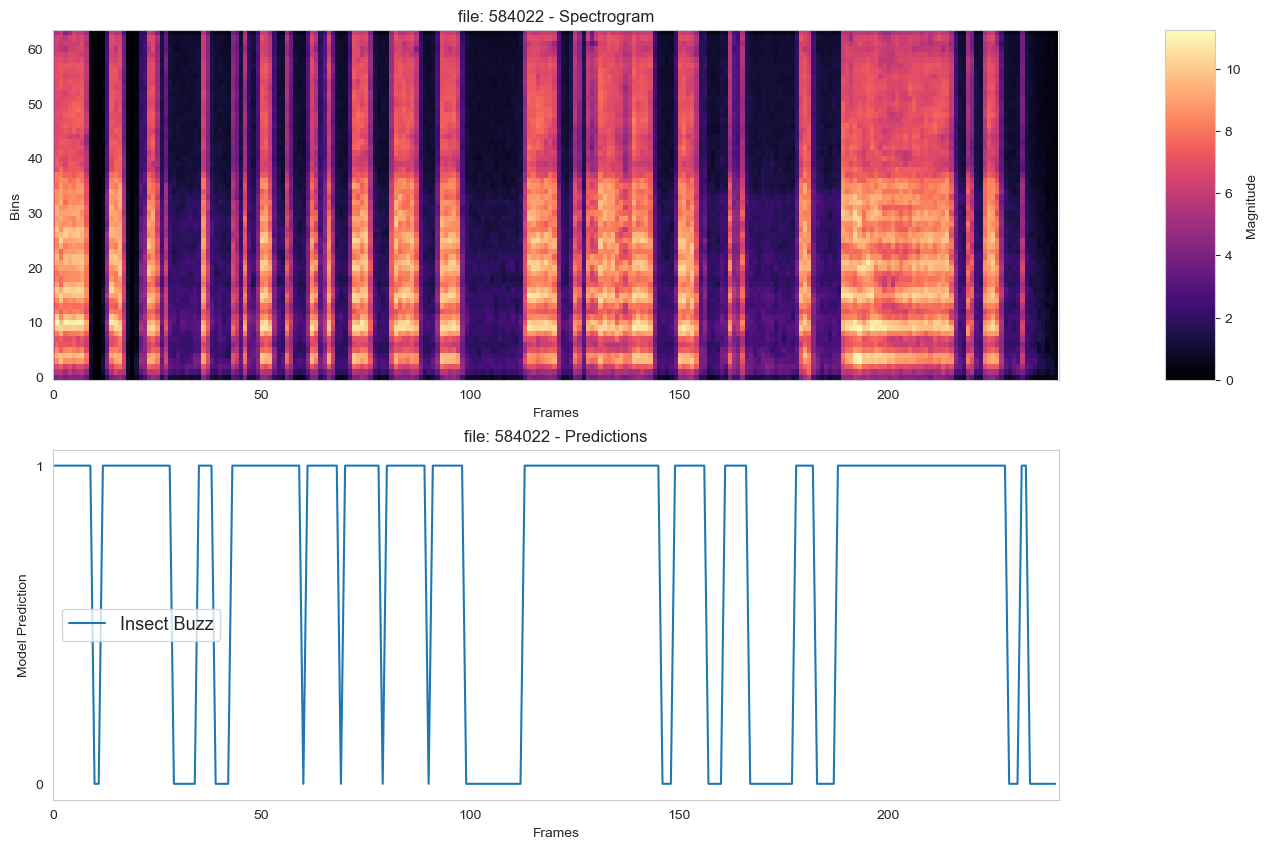
\includegraphics[width=\textwidth, height=5cm]{figs/6_good.png}
  \end{subfigure}
  \hfill
  \begin{subfigure}[b]{0.49\textwidth}
    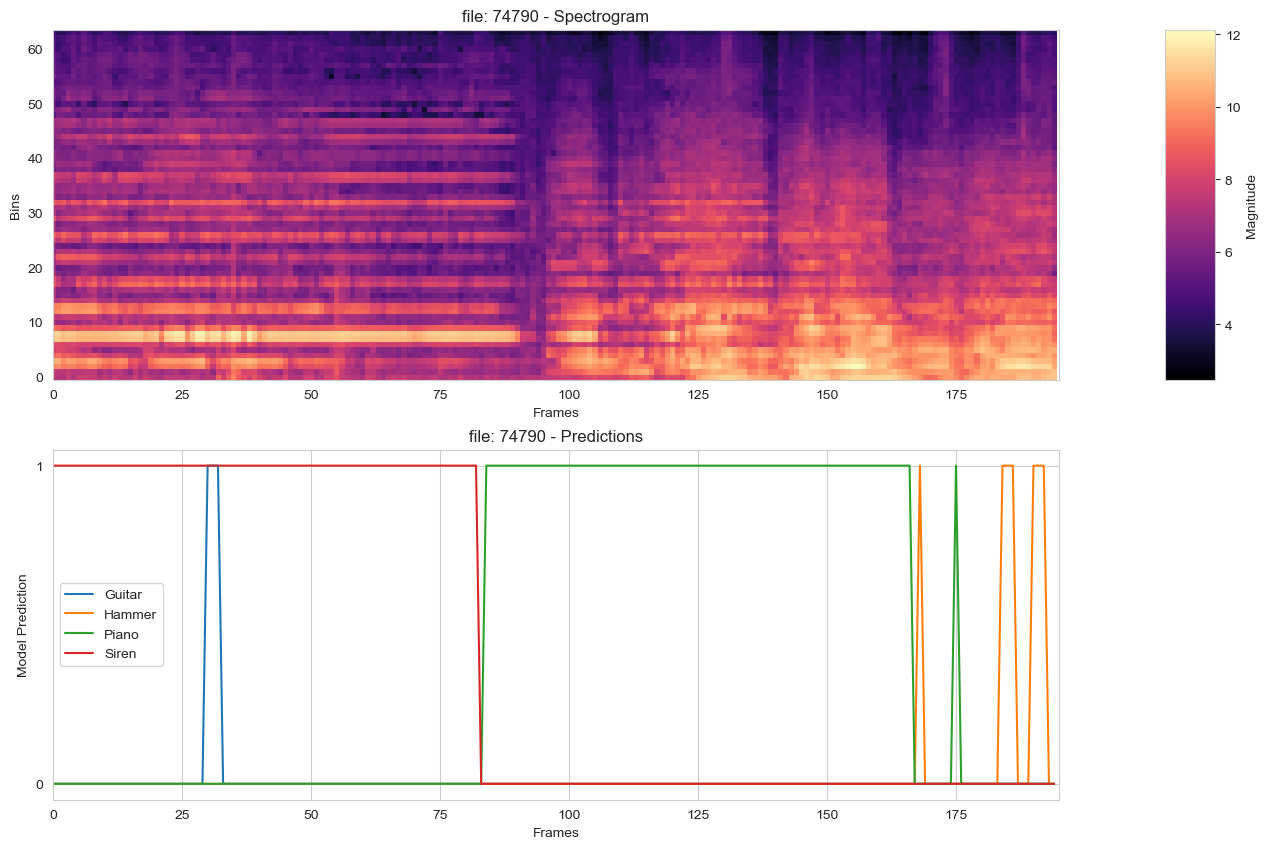
\includegraphics[width=\textwidth, height=5cm]{figs/6_bad.png}
  \end{subfigure}
  \caption{Visualization of predictions from our best model.}
  \label{fig:6_plots}
\end{figure}


\subsection{Listen to the audios and inspect the corresponding predictions of the classifier. How well does the classifier recognize the classes?}
\label{sec:Analysing Predictions:b}
\begin{itemize}
    \item \textbf{584022.wav}: This represents an extremely simple example where the models predictions are really precise and mostly correct. Not only did it correctly predict the (only) class label, but temporally the predictions match very well. Sometimes however, some of the individual buzzes get grouped together, especially when the pauses in between them get really short. The model achieved an F1-score of 0.928 and a Balanced Accuracy of 0.896 for this file.
    \item \textbf{74790.wav}: This represents a more complex example where the models predictions are horribly incorrect. When actually listening to the audio file, one clearly recognizes that it solely consists of string instruments being played and some murmuring (disregarding background noises). Confusing the strings in the beginning for a siren still is understandable, everything else is completely wrong. The model achieved an F1-score of 0 and a Balanced Accuracy of 0.25 for this file.
\end{itemize}


\subsection{What are particular problematic conditions that cause the classifier to mispredict classes? Can you think of simple postprocessing steps that might help improve the predictions?}
\label{sec:Analysing Predictions:c}

From analyzing several predictions of audio recordings we have identified that the models have a hard time predicting classes in recordings containing lots of noise or where several class labels are active at once. Additionally, predictions for class labels which are underrepresented in the dataset also are lacking. \\
Often the classifier has little peaks and valleys lasting only a few frames in its predictions, as can be seen in the second plot of \hyperref[fig:6_plots]{Figure~\ref*{fig:6_plots}} with the 'Guitar' or 'Piano' labels. Such spurious (mis-)classifications could easily be removed by setting a lower threshold for how many frames a positive or negative prediction has to last, and filtering the output accordingly. This should overall increase the quality of predictions.





